\documentclass[openright]{xmgr}
% Jeśli nowe rozdziały mają się zaczynać na stronach nieparzystych:
% \documentclass[openright]{xmgr}

\usepackage{lipsum}
\usepackage[colorinlistoftodos,prependcaption,textsize=tiny]{todonotes}
\usepackage{regexpatch}
\makeatletter
\xpatchcmd{\@todo}{\setkeys{todonotes}{#1}}{\setkeys{todonotes}{inline,#1}}{}{}
\makeatother
%\usepackage{imakeidx}
%\makeindex

% install minted package to highlight source code
% \usepackage{minted}

%\defaultfontfeatures{Scale=MatchLowercase}
%\setmainfont[Numbers=OldStyle,Ligatures=TeX]{Minion Pro}
%\setsansfont[Numbers=OldStyle,Ligatures=TeX]{Myriad Pro}
% for fontspec version < 2.0
% \setmainfont[Numbers=OldStyle,Mapping=tex-text]{Minion Pro}
% \setsansfont[Numbers=OldStyle,Mapping=tex-text]{Myriad Pro}
%\setmonofont[Scale=0.75]{Monaco}

% Opcjonalnie identyfikator dokumentu
% drukowany tylko z włączoną opcją 'brudnopis':
\wersja   {wersja wstępna [\ymdtoday]}

\author   {Dariusz Adrychowski}
\nralbumu {251682}
\email    {darek@adrychowski.com}


\title    {Wizualna inwentaryzacja znaków drogowych\todo{Uzupełnić tytuł po  uzgodnieniu}}
\date     {2018/2019}
\miejsce  {Gdańsk}

\opiekun  {dr Jakub Neumann}

% dodatkowe polecenia
%\renewcommand{\filename}[1]{\texttt{#1}}
%\definecolor{stress}{cmyk}{0,1,0.13,0} % RubineRed
%\definecolor{topic}{cmyk}{0.98,0.13,0,0.43} % MidnightBlue

\begin{document}

% streszczenie
\begin{abstract}
\todo[color=yellow]{Dodać streszczenie}
\lipsum[1-4]
\end{abstract}

% słowa kluczowe
\keywords{ słowa kluczowe }

\todo[color=blue]{uzupełnić słowa kluczowe}
% tytuł i spis treści
\maketitle

 \listoftodos

% wstęp
\introduction


Celem niniejszej pracy było stworzenie oprogramowania umożliwiającego automatyczną akwizycję obrazu, jego segmentację i wykrywanie zadanych wcześniej, zdefiniowanych obiektów --- znaków drogowych. Następnie korzystając z informacji o ich geolokalizacji, określenie ich położenia i jeśli okaże się to możliwe umieszczenia na mapie. Całość oprogramowania z założenia będzie realizowana przy użyciu kamery i wytrenowanej sieci neuronowej, która wykona detekcję i lokalizację na podstawie danych z kamery. Z założenia rozwiązanie nie musi działać online, dane geolokalizacji umieszczone będą wewnątrz zapisu wideo.
Przykładowym zastosowaniem niniejszego oprogramowania może być automatyczna inwentaryzacja znaków drogowych.

W rozdziale \ref{ch:bazowedefinicje} omówione zostały wybrane, podstawowe definicje i pojęcia wykorzystywane w niniejszej pracy. W rozdziale \ref{ch:historia} przedstawiono krótki rys historyczny klasyfikacji i wykrywania obiektów w obrazie wideo i omówiono podstawowe metody realizacji powyższych. Rozdział \ref{ch:preprocesing} zawiera omówienie procesu przetwarzania danych od momentu ich pozyskania, czyszczenie po ich przygotowanie do procesu trenowania sieci. Rozdział \ref{ch:realizacja} zawiera szczegółowy opis procesu tworzenia sieci --- od wyboru sprzętu za pomocą którego zrealizowano zadanie, poprzez trenowanie sieci po finalne przetwarzanie i wykrywanie obiektów. Rozdział \ref{ch:analizawynikow} zawiera opis analizy pozyskanych wyników, zawiera również krótkie rozważania na temat możliwych przyszłych prac nad udoskonaleniem pracy. Rozdział \ref{ch:zakonczenie} zawiera podsumowanie i wnioski końcowe do jakich doszedł autor po wykonaniu niniejszej pracy.

\chapter{Bazowe definicje} \label{ch:bazowedefinicje}
\subsection*{} \noindent Poniższy rozdział zawiera opis podstawowych pojęć używanych w niniejszej pracy --- ich definicję, skróconą historię i krótki opis.

\section{Sieci neuronowe i algorytmy}

W chwili pisania tej pracy do klasyfikacji i detekcji obiektów na obrazie wykorzystywano kilka różnych sieci neuronowych. Sieci te wykorzystują kilka bazowych algorytmów --- wybór regionów obrazu do analizy jest decydującym czynnikiem dla każdego z algorytmów.
 
\subsection{R---CNN Region---Convolutional Neuron Network}

Sieci typu R-CNN zostały stworzone w celu umożliwienia szybkiej detekcji obiektów, ich lokalizacji i klasyfikacji. Sygnałem wejściowym podawanym wytrenowanej sieci jest obraz. Odpowiedzią sieci R-CNN jest zestaw koordynat ramek (ang: bounding boxes) obejmujących wykryte obiekty oraz nazwa klasy do której je zakwalifikowano. Algorytm ewoluował z sieci CNN kolejno do:
\begin{itemize}
	\item R---CNN
	\item Fast---R---CNN
	\item Faster---R---CNN
\end{itemize}

Głównymi problemami blokującymi możliwość wykorzystania sieci typu R---CNN do detekcji obiektów w czasie rzeczywistym między innymi:
\begin{itemize}
	\item trenowanie sieci jest skomplikowane i zabiera bardzo dużo czasu
	\item trening odbywa się w wielu fazach (np.: trening klasyfikacji versus nauka wyboru odpowiednich regionów do obróbki)
	\item sieć jest bardzo wolna na etapie wnioskowania (szczególnie kiedy ma do czynienia z danymi, które nie były objęte szkoleniem)
\end{itemize}

\subsection{SSD --- Single Shot MultiBox Detector}
Algorytm opracowany przez C. Szegedyat al.\cite{DBLP:journals/corr/LiuAESR15} na przełomie roku 2016/2017. Dedykowany do szybkiej detekcji obiektów w obrazie wideo. Nazwa algorytmu wzięła się od z opisu jego działania:
\begin{itemize}
	\item Single Shot - lokalizacja obiektu i jego klasyfikacja wykonywana jest w jednym przebiegu sieci
	\item MultiBox - nazwa techniki opracowanej przez Szegedy'ego et al. 
	\item Detector - sieć jest detektorem obiektów i wykonuje ich klasyfikacji
\end{itemize}

Sieci SSD budowane są w architekturze opartej na modelu VGG-16, bez warstw fully connected. Głównym powodem użycia VGG-16 jako sieci wyjściowej była wydajność tego modelu i jak również popularność (dostępność wielu modeli gotowych do transfer learning). 
W budowie sieci zamiast warstw fully connected zastosowano zestaw konwulcyjnych warstw pomocniczych --- właściwa detekcja odbywa się w większej skali progresywnie zmniejsza rozmiar wejść do każdej następnej warstwy.
\begin{figure}[ht]
	\centering
	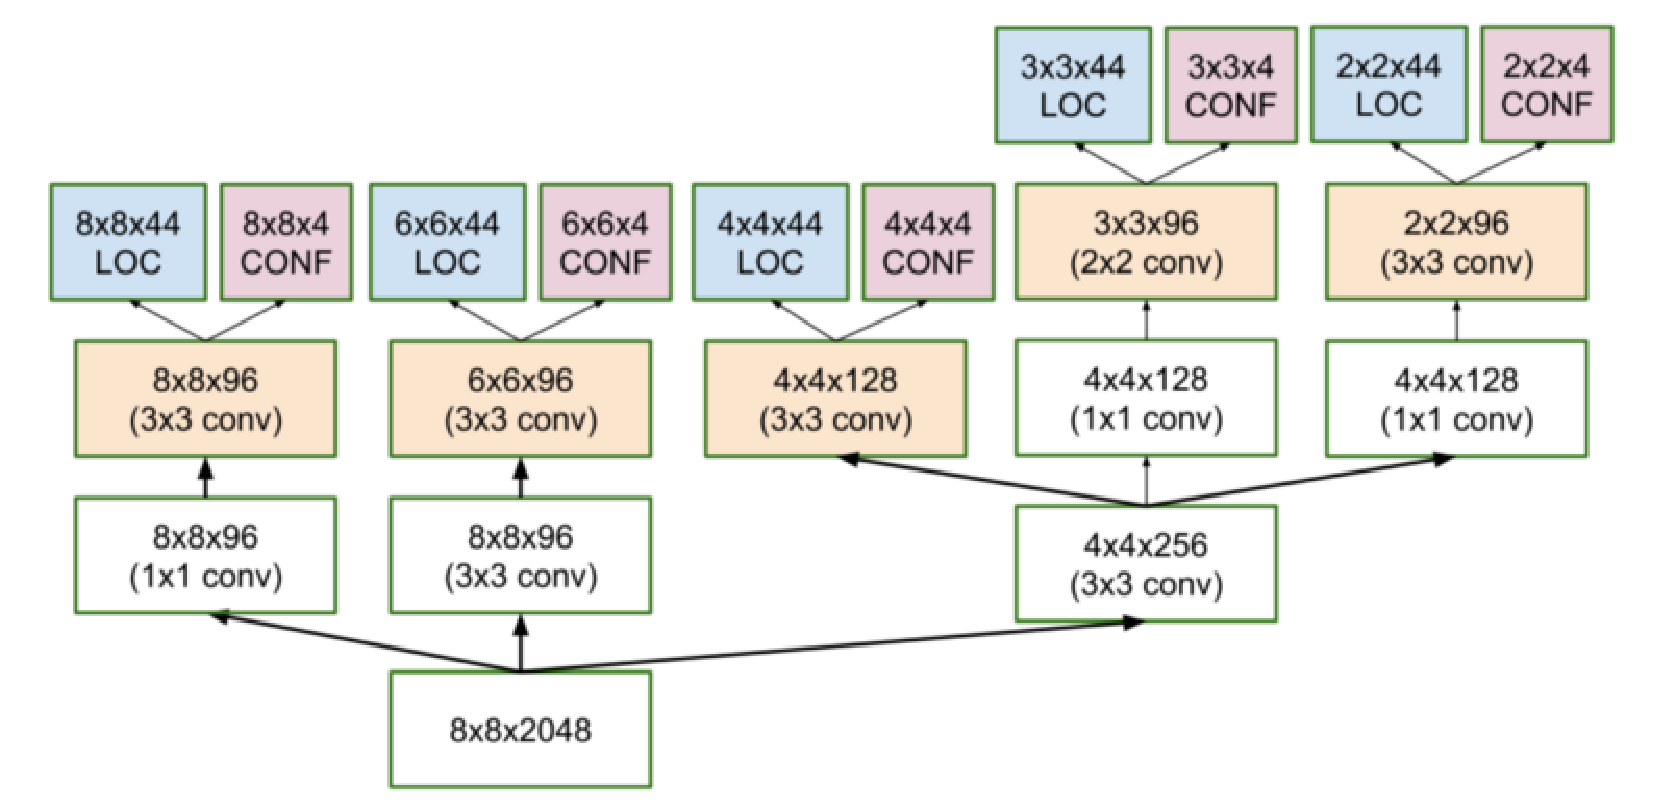
\includegraphics[width=\textwidth]{fig/ssd.pdf}
	\caption{Budowa wielkoskalowego konwulsyjnego przewidywania lokalizacji multiboksów. źródło: \cite{DBLP:journals/corr/LiuAESR15}}
	\label{fig:ssd}
\end{figure}

Technika  MultiBox wytycza szybko koordynaty ramek (bounding boxes) otaczających obiekty bez wiedzy o ich klasie. Rys \ref{fig:ssd} pokazuje w jaki sposób redukowany jest liczba wymiarów ramek.


\subsection{Framework'i}
Algorytmy implementowane są w różnych wariantach i dostępne jako gotowe biblioteki w kilku framework\'ach.\todo{uzupełnić: Theano, Keras, Tensorflow, Detectron}

\subsection{Architektura sieci}

\subsubsection{AlexNet}
Historycznie biorąc AlexNet jest pierwszą z sieci neuronowych wykorzystywanych do detekcji obiektów w obrazie wideo, która była znacząco podnieść poziom dokładności wykrywania w rankingu ImageNet Classification. Składa się ona z 5 konwulcyjnych warstw i następujących po nich trzech w pełni połączonych warstw. Struktura zaproponowana przez Alex\'a Krizhevsky\'ego wyróżniała się również zastosowaniem funkcji aktywacji ReLu (Rectified Linear Unit) zamiast tradycyjnie stosowanych funkcji tangens hiperboliczny czy sigmo-idów.
ReLu definiowana jest jako:
\begin{equation} \label{eq:relu}
f(x)=max(0,x)
\end{equation}
Dużą przewagą funkcji \ref{eq:relu} nad poprzednio powszechnie używanymi funkcjami (tanh i sigmoid) jest szybkość uczenia się. Dzieje się tak dlatego, że po przekroczeniu pewnej wartości zarówno funkcja tanh jak i sigmoid wchodzi w stan nasycenia i zmiany impulsu wejściowego nie powodują, bądź powodują bardzo małe zmiany na wyjściu --- stan ten jest nazywany problemem zanikającego gradientu (ang.: vanishing gradient problem)
\begin{figure}[htp]	
	\centering
	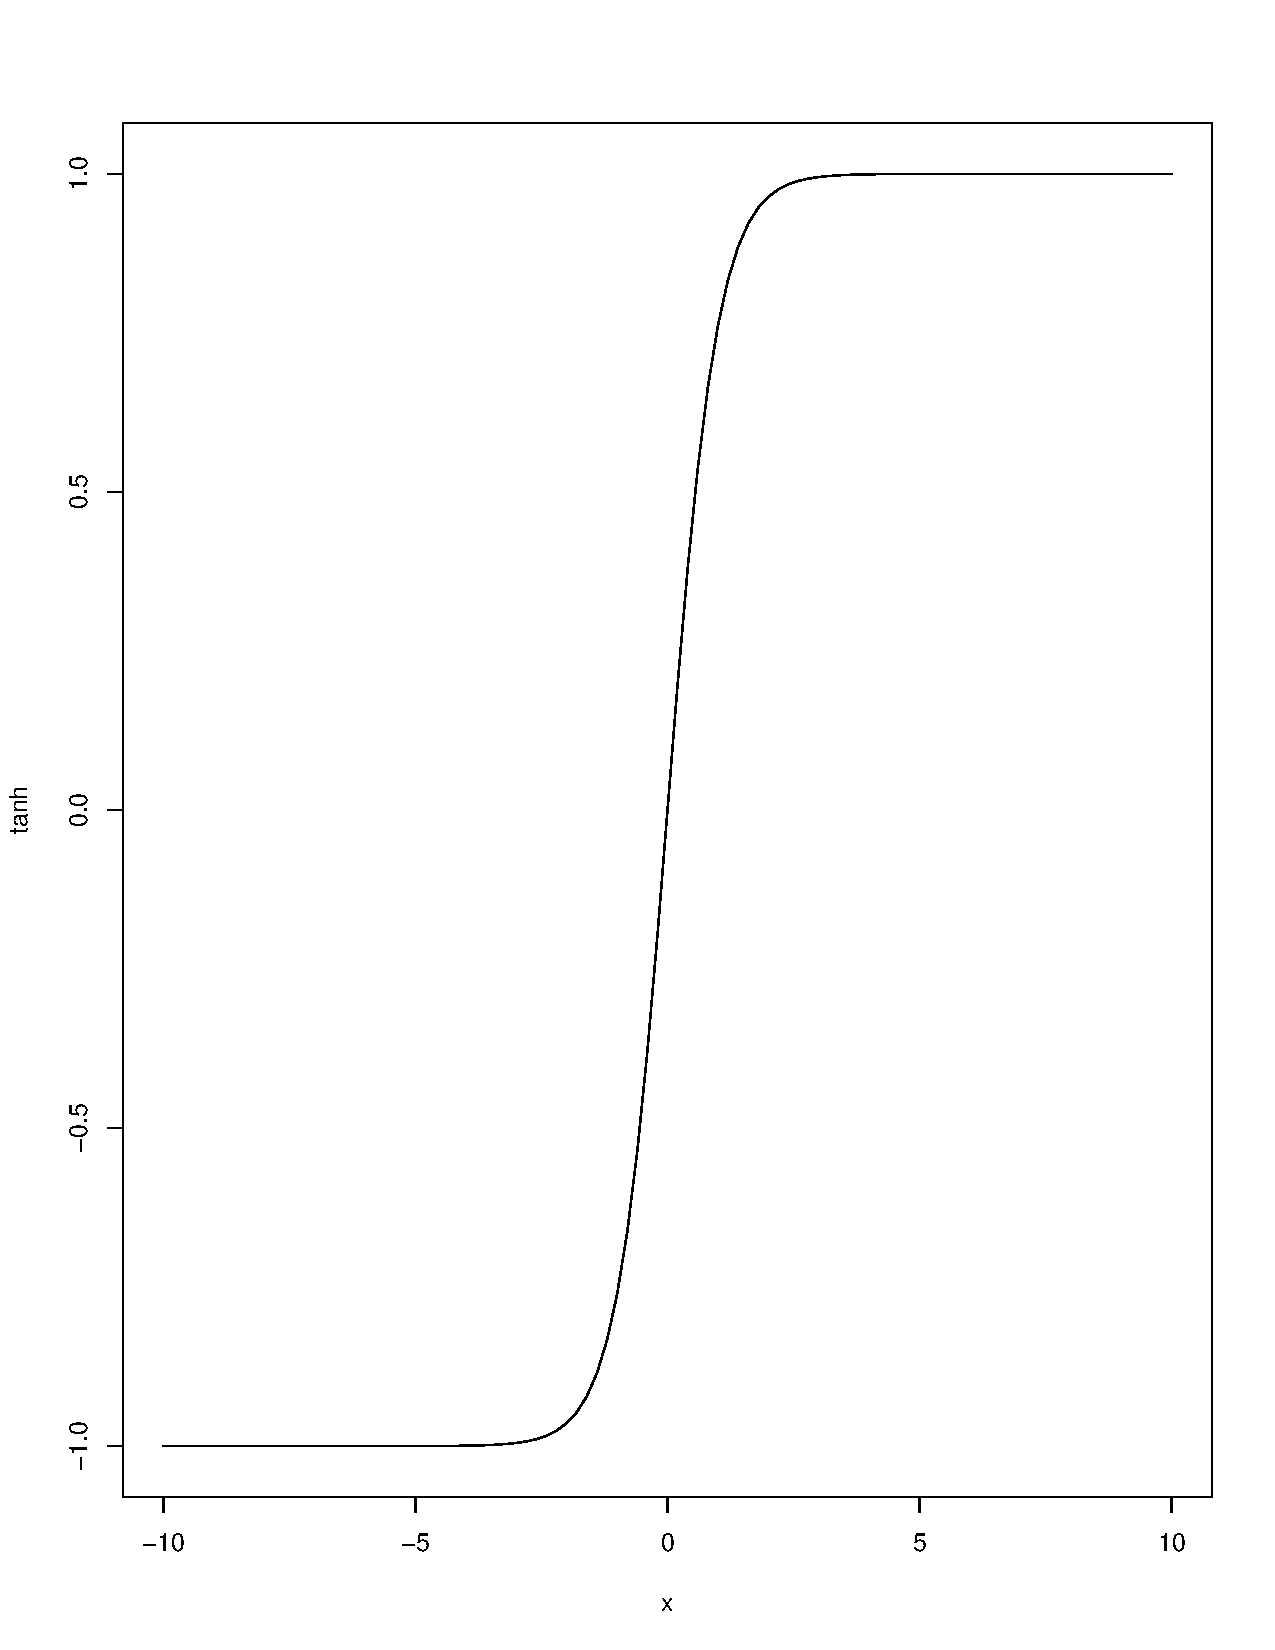
\includegraphics[width=.3\textwidth]{fig/tan.pdf}\hfill
	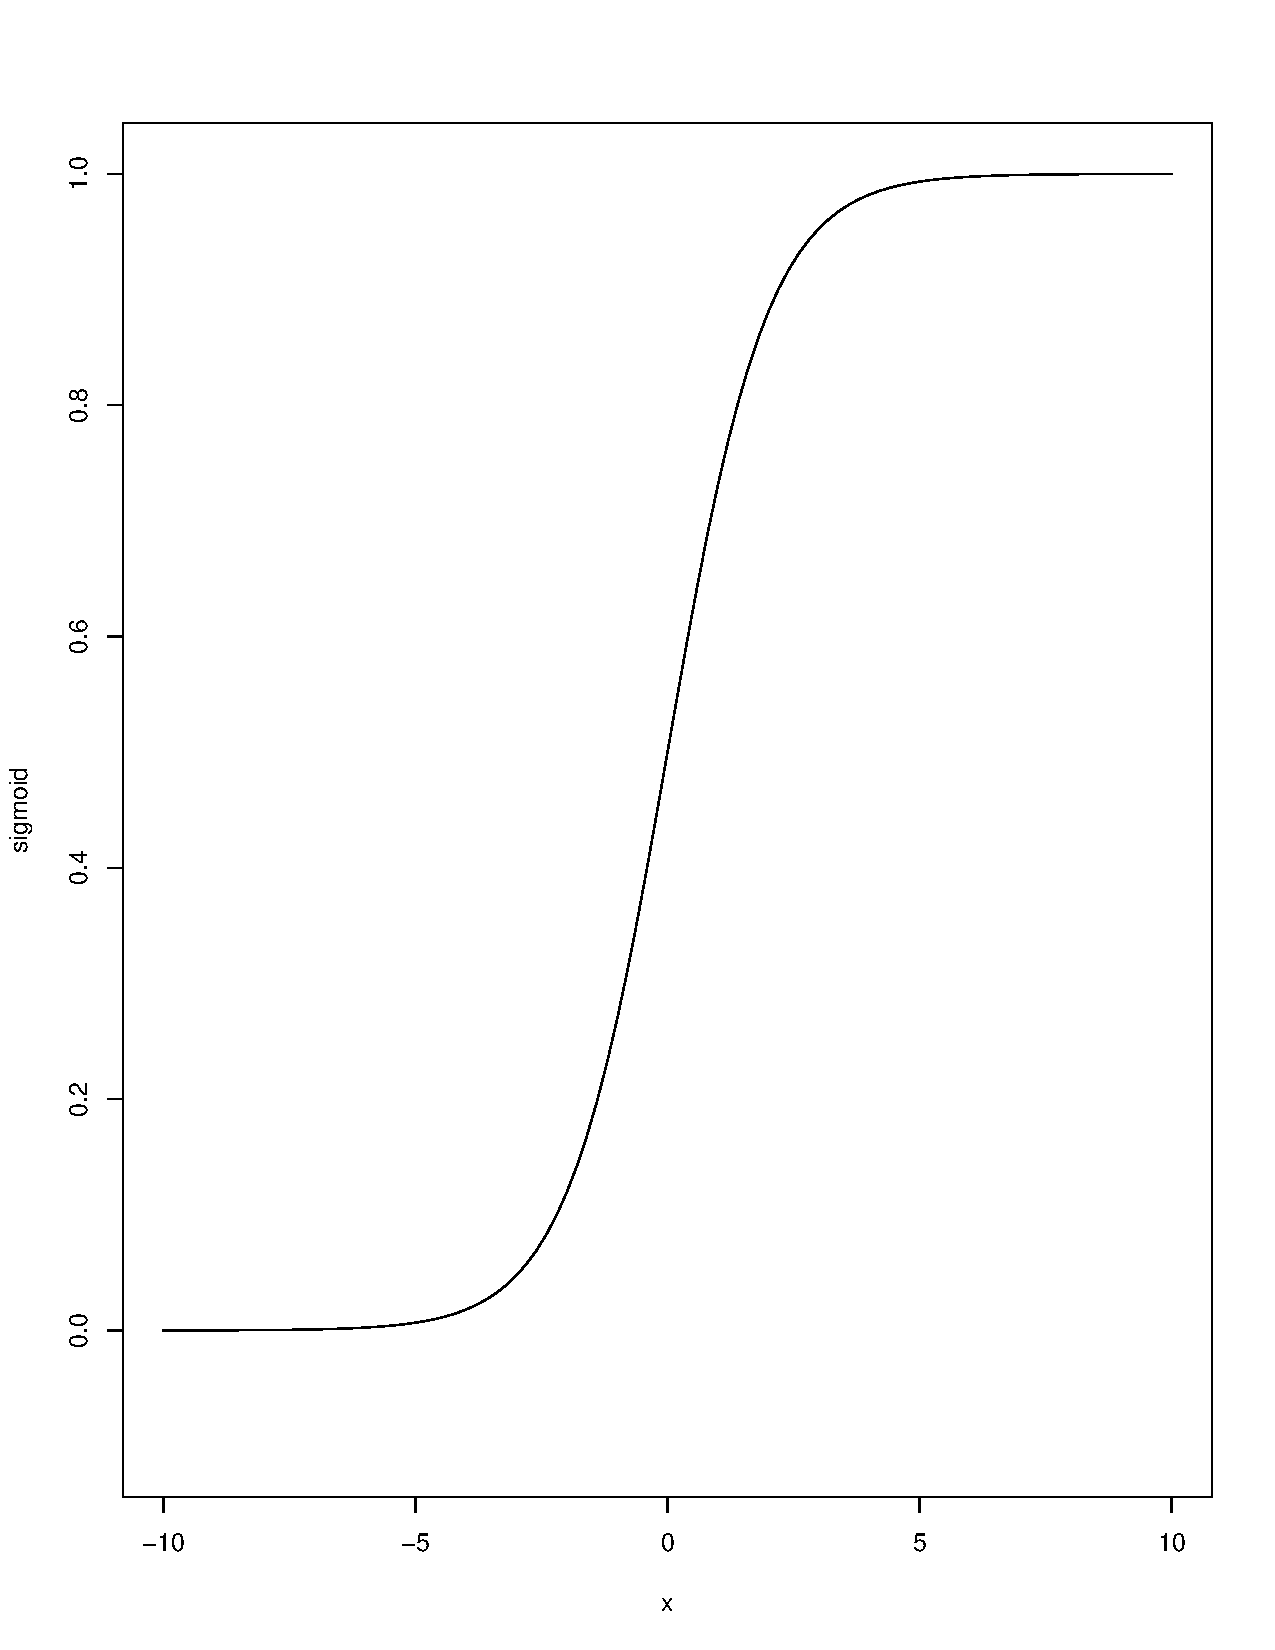
\includegraphics[width=.3\textwidth]{fig/sigm.pdf}\hfill
	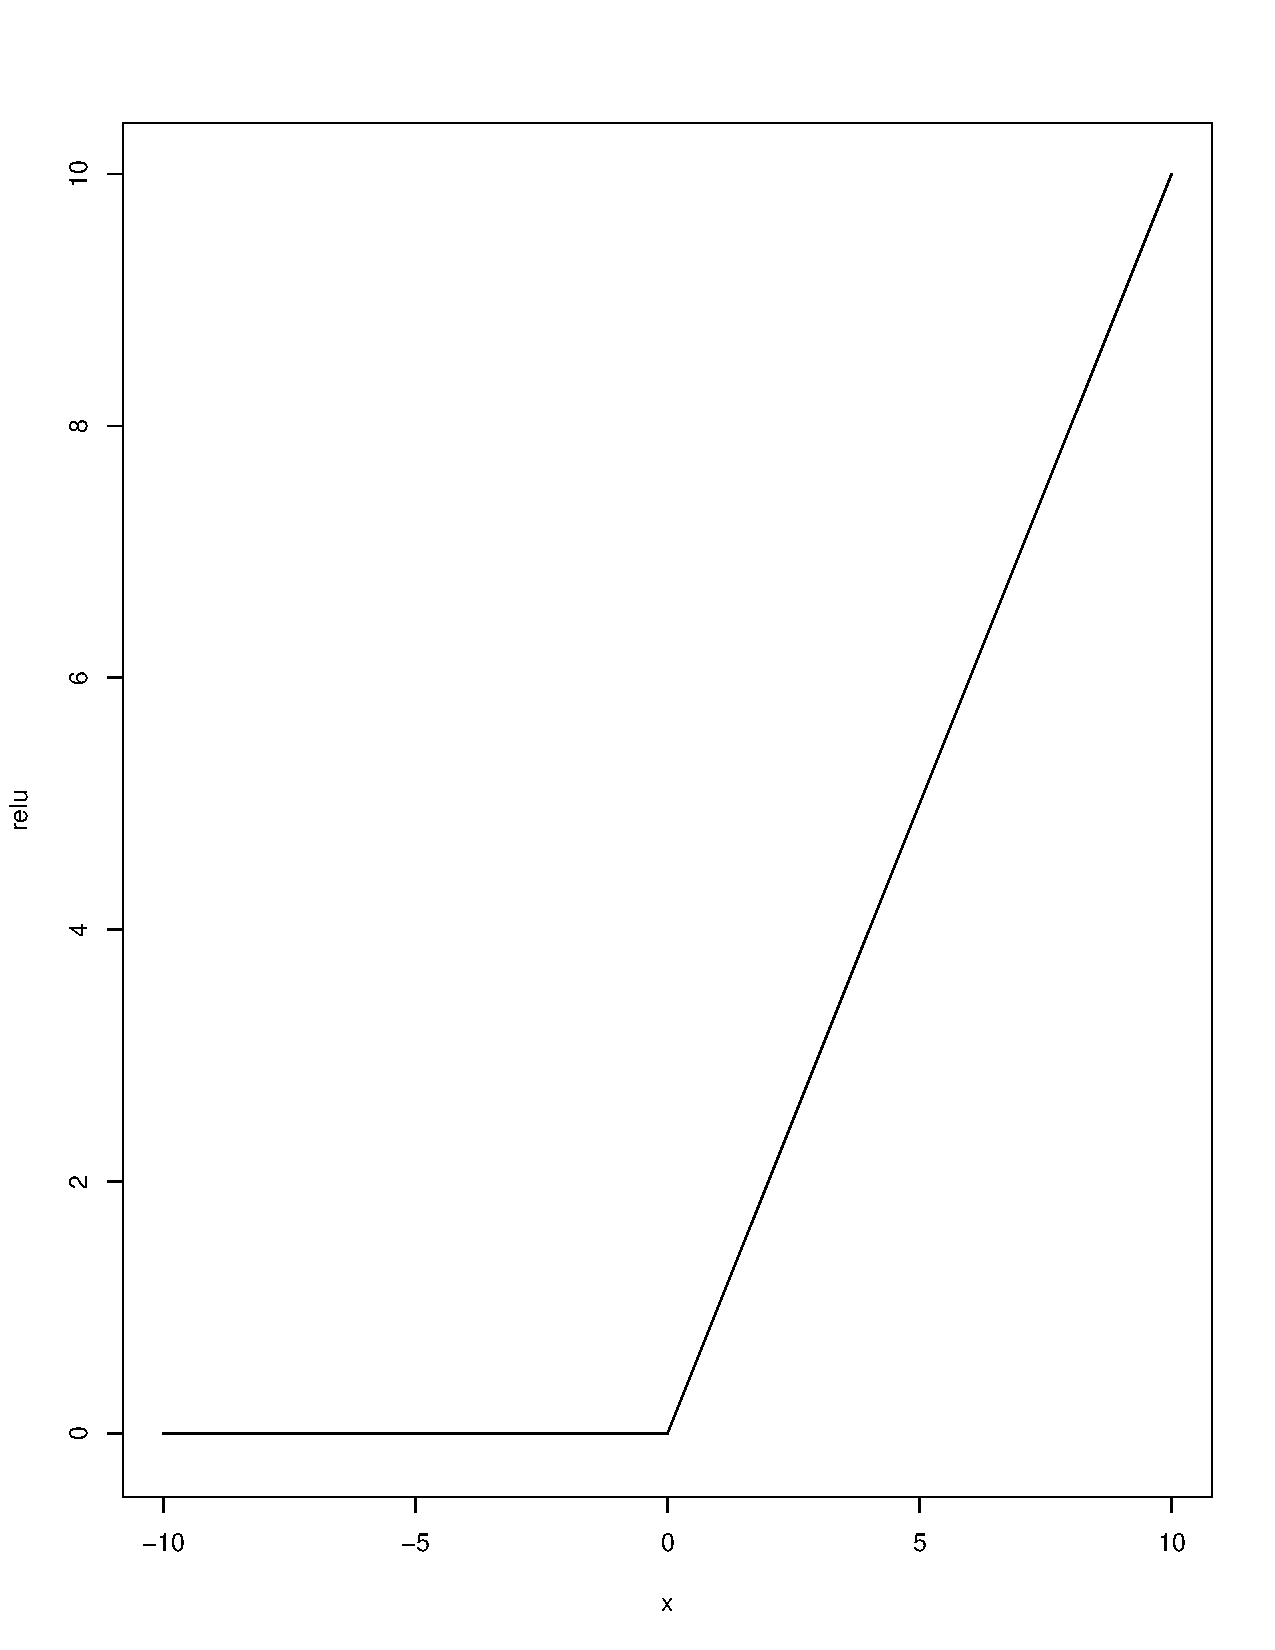
\includegraphics[width=.3\textwidth]{fig/relu.pdf}	
	\caption{Funkcje aktywujące: kolejno tangens hiperboliczny, sigmoid, ReLu}
	\label{fig:relu}	
\end{figure}
Dodatkowo, aby ograniczyć przetrenowanie sieci po każdej warstwie w pełni połączonej dodano warstwę Dropout --- każdy neuron z określonym prawdopodobieństwem $p$ może zostać wyłączony. 

\subsubsection{VGG---16}
Grupa VGG z Oxfordu udoskonaliła AlexNet poprzez usunięcie dużych filtrów i zastąpiła je wieloma filtrami mniejszymi. Z jednej strony zmiejszyło to potrzebny nakład mocy obliczeniowej, z drugiej zwiększył głębokość sieci --- co za tym idzie zdolność do nauki bardziej skomplikowanych schematów.

\subsubsection{GoogLeNet/Inception}\cite{43022}
Ponieważ VGG---16 cechowała niezwykła dokładność przy bardzo dużym nakładzie mocy obliczeniowej i pamięci potrzebnej do zaimplementowania sieci, Google rozpoczęło prace nad udoskonaleniem modelu VGG. Rezultatem tego jest właśnie GoogLeNet --- cechą charakterystyczną jest warstwa wejściowa (Inception)\cite{ai_gitbook}. Warstwa Inception aproksymuje rzadką sieć CNN z sieci o normalnej gęstości. Z właściwości złożonych sieci neuronowych wynika, że tylko niewielka ilość neuronów jest skuteczna -- ilość filtrów jest również redukowana. Do wychwycenia detali aplikowane są filtry o różnych wielkościach i o różnej skali. 
\begin{figure}[htp]	
	\centering
	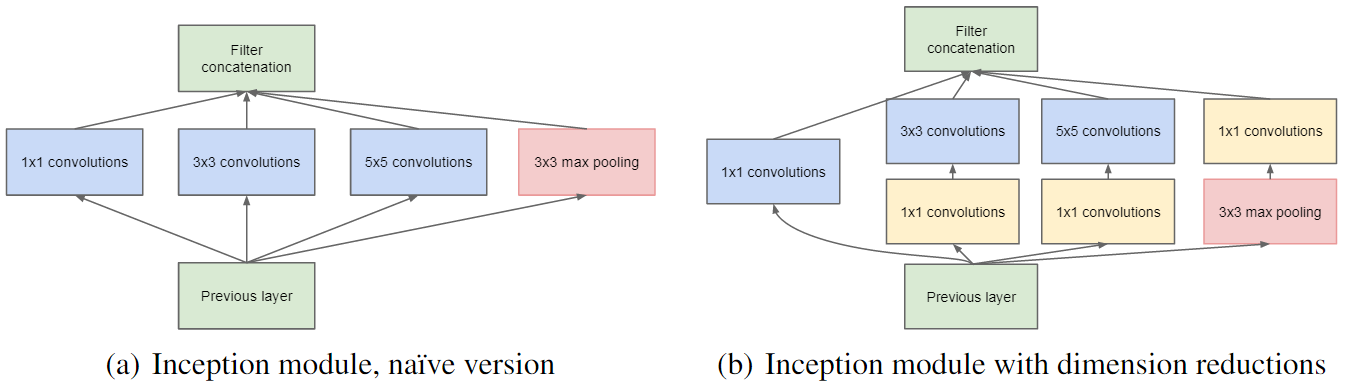
\includegraphics[width=.3\textwidth]{fig/inception_1x1.png}\hfill
	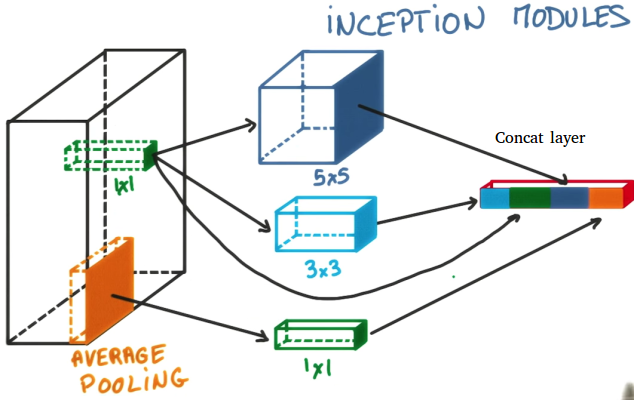
\includegraphics[width=.3\textwidth]{fig/InceptionModules.png}\hfill
	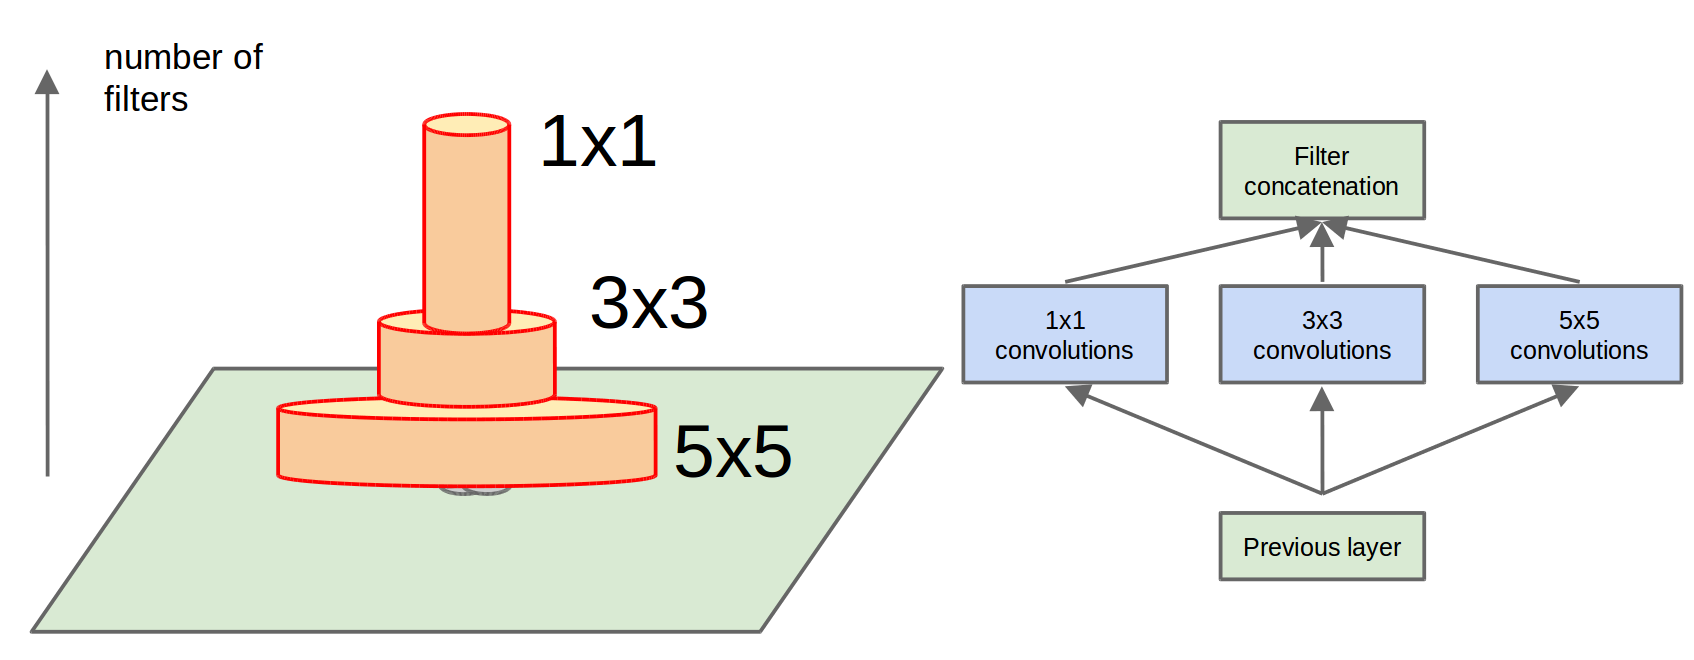
\includegraphics[width=.3\textwidth]{fig/Naive_VersionNception.png}	
	\caption{GoogLeNet}
	\label{fig:GoogLeNet}	
\end{figure}


\subsubsection{Residual Networks}
Zwiększanie głębokości sieci neuronowej (ilości warstw ukrytych) prowadzi do zwiększenia dokładności sieci jeśli zwracamy dużą uwagę na przetrenowanie sieci i do niej nie doprowadzimy. Im większa głębokość sieci, tym sygnał potrzebny do zmiany wag jest mniejszy. Maleje on wraz z ilością warstw. Łatwo zauważyć, że pierwsze warstwy tracą na ważności -- zjawisko to nazywa się zanikającym gradientem. Oczywiście optymalizacja głębokiej sieci jest też dużo bardziej skomplikowana ze względu na ilość współczynników wag do dostrojenia.Problemy te częściowo rozwiązują sieci rezydualne.
Sieci rezydualne usprawniają szkolenie głębokich sieci poprzez zastosowanie modułów zwanych modułami rezydualnymi.
\begin{figure}[ht]
	\centering
	\includegraphics[width=\textwidth]{fig/res1.png}
	\caption{Zasada nauki sieci głębokich przy użyciu modułów rezydualnych}
	\label{fig:residual1}
\end{figure}

\subsubsection{}
next sub
\subsection{Wykrywanie vs klasyfikacja}

\subsubsection{Wykrywanie}
Wykrywanie obiektów wykorzystuje algorytmy klasyfikujące do określenia co i gdzie znajduje się na badanych obrazie (również wideo). Powstanie i rozwój sieci CNN umożliwiło wyrywanie wielu klas przy pojedynczej analizie. Algorytm wykrywający (ang. object detection) po zbadaniu obrazu przedstawi rozmieszczenie na obrazie rozpoznanych obiektów.

\subsubsection{Klasyfikacja}
Klasyfikacja polega na określeniu czy obraz należy do pewnej, z góry określonej kategorii. Np. klasyfikator odpowiada na pytanie --- czy na badanym obrazie znajduje się kot.

\section{Transfer Learning}

Transfer learning jest zbiorczą nazwą na zestaw technik służących do ponownego użycia i zmiany wyuczonego tematu do rozpoznawania nowego w celu przyspieszenia procesu trenowania sieci neuronowej. Ponieważ tworzenie i uczenie sieci neuronowej wymaga zaangażowania znacznych mocy obliczeniowych, a wykorzystanie transfer learning znacznie obniża to wymaganie jest to technika bardzo popularna i chętnie wykorzystywana w procesie uczenia maszynowego. Aby przyspieszyć i ułatwić ten aspekt pracy z sieciami neuronowymi stworzono zestawy narzędzi ułatwiających to zadanie. Jako przykład posłużyć może dostępna na licencji Apache 2.0 biblioteka Xfer do pobrania z repozytorium Github\cite{xfer_git}.\\

Sieci neuronowe posiadają właściwość nauki korelacji pomiędzy sygnałem wejściowym (np.: obrazem) a jego reprezentacją (np.: opisem). Proces takiej nauki nazywany jest uczeniem nadzorowanym. Po wytrenowaniu sieć jest zdolna do przewidywania powiązania pomiędzy sygnałem wejściowym i najbardziej pasującą reprezentacją. Niestety, jeśli warunki brzegowe w czasie implementacji mogą ulec zmianie lub sieć ma zostać wykorzystana do wykrywania innego rodzaju danych. Np.: sieć wytrenowana do rozpoznawania samolotów w grze komputerowej --- zaaplikowana w aplikacji identyfikującej samoloty z kamery operującej na prawdziwym lotnisku. Sieć może nie znać części samolotów, nie będzie ich więc w stanie rozpoznać, w świecie rzeczywistym na jakość sygnału wejściowego będą miały wpływ warunki atmosferyczne itp..
Aby zapewnić wyższą skuteczność rozpoznawania sieć powinna zostać wytrenowana na danych, na których ma pracować. Bardzo często nie jest to możliwe, bądź nie jest opłacalne ze względu na wymagany czas, nakłady mocy obliczeniowej... Możliwy i częsty jest scenariusz, w którym nie dysponujemy odpowiednio duża ilością przykładów do nauki sieci. W omawianym przykładnie może to być np.: przygotowanie się do rozpoznawania samolotów w warunkach ciężkiej zimy posiadając ograniczoną ilość zdjęć samolotów w czasie śnieżycy. W takich właśnie przypadkach wykorzystanie transfer learning jest najbardziej wskazane. Pomimo, że oryginalnie rozpoznawane obiekty i nowe są różne, posiadają one zawsze jakieś cechy wspólne (powinny takie posiadać). W takim przypadku sieć może kontynuować przerwaną naukę, bazując na elementach wspólnych wykrywanych obiektów.\\

Podsumowując słowami Andei'a Karpathy\cite{karpathy:CS231}: praktycznie niewiele osób trenuje całą sieć konwulsyjną (Convutional Network) od początku (z losową inicjlizacją wag sieci) ze względu na brak zestawu danych odpowiedniej wielkości. Zamiast tego wykorzystywane są wytrenowane na dużych zestawach danych modele, które de-facto inicjalizują wagi sieci docelowej.







\chapter{Istniejące rozwiązania i historia rozwoju detekcji obiektów w obrazie wideo} \label{ch:historia}
\subsection*{} \noindent Poniższy rozdział zawiera opis istniejących rozwiązań komercyjnych i niekomercyjnych, z którymi autor miał okazję zapoznać. Dodatkowo dołączono krótką historię rozwoju i opisano sposób wykorzystania ich w trakcie opracowywania rozwiązania będącego tematem niniejszej pracy.

\section{Detekcja obiektów w obrazie wideo}
„Deep Learning” koncentruje się na pięciu podstawowych domenach --- klasyfikacja obrazów, rozpoznawanie mowy, semantyczna klasyfikacja tekstów i rozpoznawanie / detekcja obiektów w obrazie wideo. Z punktu widzenia formalnego wideo jest tylko sekwencją obrazów zmieniających się wraz z upływem czasu. Podejście takie zakwestionował i udokumentował Andej Karpathy --- obecnie [styczeń 2019] zatrudniony jako Director of AI at Tesla.
Jego praca ''Large-scale Video Classification with Convolutional Neural Networks''\cite{KarpathyCVPR14} opisuje sposób detekcji obrazu wideo podobnie do detekcji obiektów \index{CNN}CNN\footnote{CNN --- Convolutional Neural Networks} dla modelowego obrazu. Praca ta jest jakby punktem przełomowym w dziedzinie przetwarzania obrazu --- wcześniejsze rozwiązania bazowały na opisywaniu sklasyfikowanego obrazu zestawem słów go reprezentującym (klasyfikacja)\footnote{bag of words} i decydowaniu przy użyciu algorytmu k-means %\index{k-means} 
oraz SVM %\index{SVM}
\footnote{SVM --- Support Vector Machines} o treści obrazu. Artykuł przedstawia podstawy integracji wszystkich wcześniejszych technik w jeden model CNN. Podejście do analizy obrazu wideo poprzez podzielenie jej na trzy komponenty miało wpływ na wszystkie późniejsze algorytmy przetwarzania obrazu:
\begin{itemize}
    \item połączenie elementów w dziedzinie czasu (interakcje, zmiany i przekształcenia)
    \item adaptatywny rozmiar analizowanego regionu
    \item transfer learning\index{transfer learning}
\end{itemize}
%1st d

Aby zmniejszyć ilość potrzebnej pamięci do budowania modelu, Karpathy ze swoim zespołem jednocześnie przetwarzał tylko jeden film, dodatkowo wstępna obróbka była przeprowadzana na różnych maszynach. Aby zapewnić jednakową długość danych wejściowych klipy pochodzące z YouTube podzielono na półsekundowe sekwencje. Agregacja przewidywanych półsekundowych klipów przypomina testowanie klasyfikacji w dziedzinie czasu - w przypadku obrazu  klatka z początku klipu nawet przedstawiając ten sam obraz po pół sekundzie będzie przedstawiała ten sam obraz po pewnej transformacji. Obiekt na obu klatkach może zostać odkształcony w wyniku przemieszczenia się czy to samego obiektu czy też kamery (przekształcenia izomorficzne), jak również mogą ulec zmianie warunki w których wykonywane jest nagranie (wiatr, deszcz, nasłonecznienie itp.).
Karparhy et al. przedstawiają również nowe podejście do dziedziny czasu (w momencie publikacji) --- aplikują zasady opisujące sieci konwulsyjne do dziedziny czasu i zależności czasowych w wideo. Grupa ramek jest składana razem (grupowana) i staje się obrazem wejściowym do sieci CNN %\index{CNN}. 
Standardowa sieć CNN jako wejście otrzymuje macierz danych --- wysokość, szerokość i kolor (wartości w każdym z trzech składowych). Karpathy i jego zespół rozszerzyli parametry wejściowe i wcześniejszą ramkę umieścili na obecnej --- zachowując rozmiary przekazują podwójną informację o kolorze --- dla obu ramek osobno. Ze względu na scalanie ramek, Karpathy et al. zaproponowali różne strategie realizacji przy założeniu klasyfikowaniu jednej ramki (kombinowanej) jednocześnie. W zależności od tego, które ramki są składane, zespół osiągnął inne rezultaty. Poniższy rysunek przedstawia przyjęte strategie.\\
\begin{figure}[ht]
    \centering
    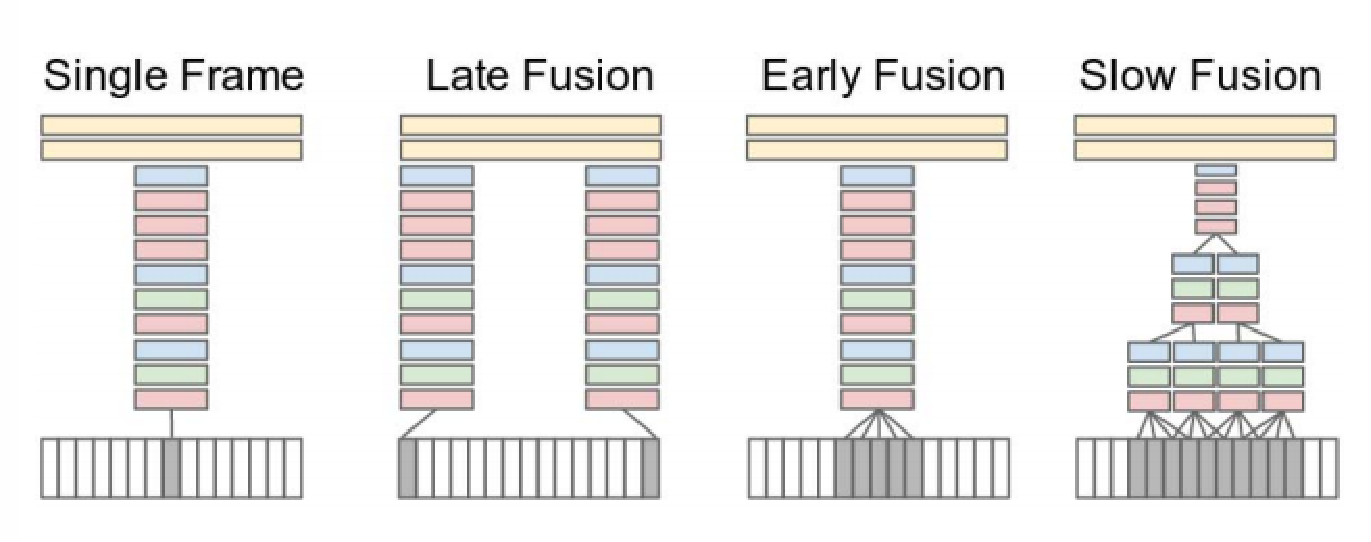
\includegraphics[width=\textwidth]{fig/karpathy1.pdf}
    \caption{Strategie przetwarzania ramek zaproponowane przez Karpathy et al. źródło: ''Large-scale Video Classification with Convolutional Neural Networks''}
    \label{fig:karpathy1}
\end{figure}
\begin{itemize}
\item Model Single Frame z rysunku \ref{fig:karpathy1} reprezentuje wcześniejszy sposób przetwarzania/ klasyfikacji obrazu wideo --- pojedyncza ramka jest interpretowana jak statyczny obraz, informacja temporalna nie jest uwzględniana. 
\item Late Fusion grupuje i scala ramki skraje z zadanego przedziału czasu --- na ostatnią ramkę nakłada się ramkę pierwszą.

\item Early Fusion grupuje kilka ramek z ciągłego przedziału czasu.
\item Slow Fusion jest najbardziej skomplikowanym modelem --- cztery częściowo nakładające się na siebie grupy ramek (ovelapping równy jest dwie ramki) wybrane z ciągłego przedziału czasu są przekształcane przez sieć.
\end{itemize}
W wyniku eksperyment stwierdzono, że Slow Fusion dostarcza najbardziej użyteczną informację o obrazie, jednak jakość ta nie była dużo większa od jakości informacji otrzymanej z modelu Single Frame. Najlepsze wyniki dawało uśrednienie informacji pochodzącej ze wszystkich rozpatrywanych modeli (Single + Early + Late + Slow).
W omawianej pracy przedstawiono również koncept przetwarzana obrazu sieci CNN wielu rozdzielczości.
\begin{figure}[ht]
    \centering
    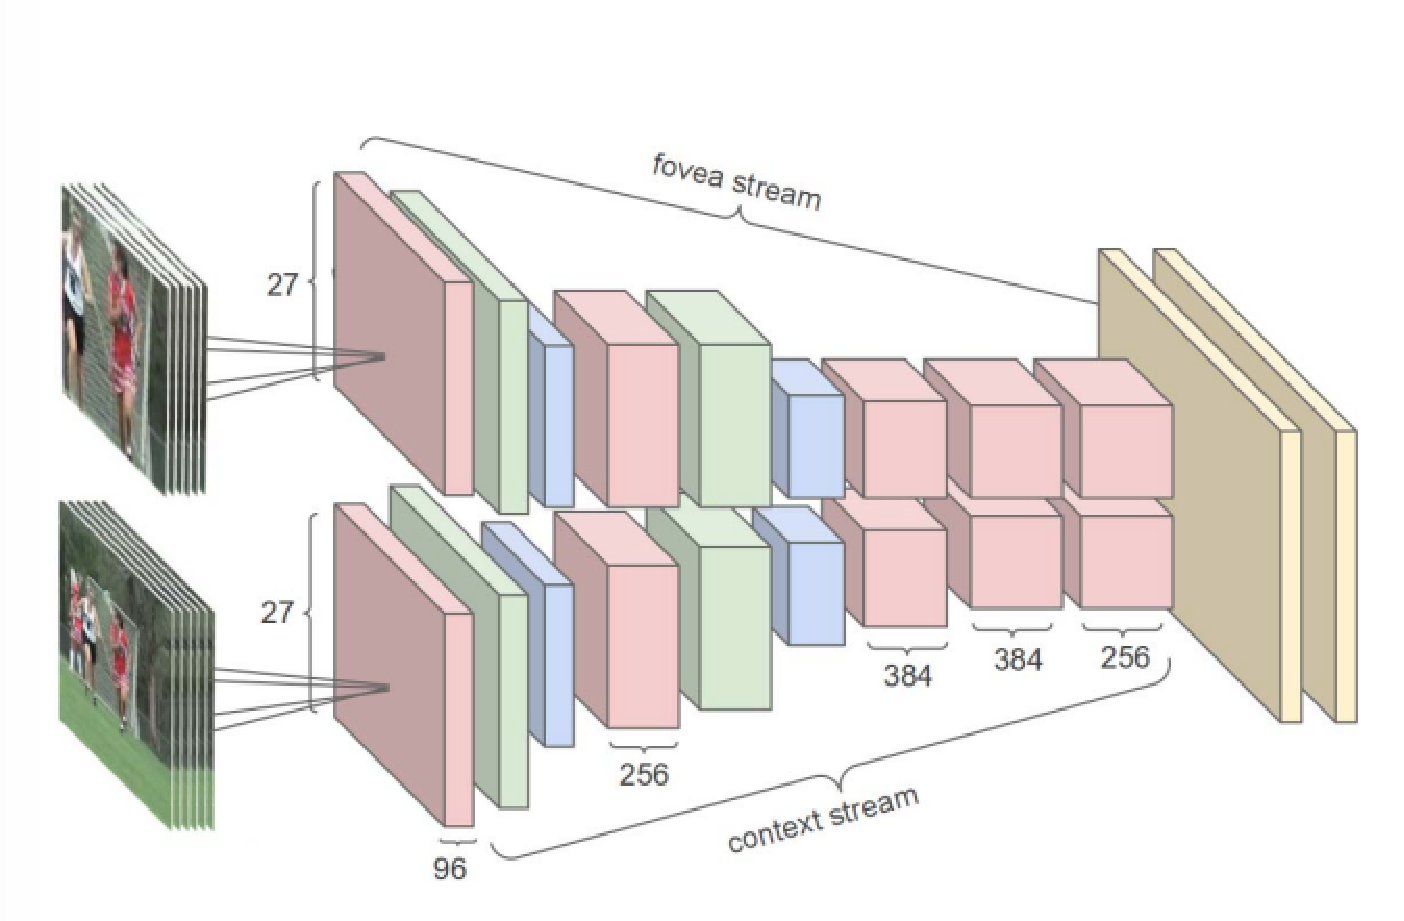
\includegraphics[width=\textwidth]{fig/multi_res.pdf}
    \caption{Strategia klasyfikowania obrazu przez sieci CNN o wielu rozdzielczościach źródło: ''Large-scale Video Classification with Convolutional Neural Networks''}
    \label{fig:multi_resKa}
\end{figure}

Zasada działania przedstawiona na rysunku \ref{fig:multi_resKa} --- dwa odrębne wejścia przetwarzają obraz przez odrębne sieci.

Pomysł przetwarzania wątków o kilku rozdzielczościach polega na jednoczesnym podaniu na wejściu odrębnych sieci neuronowych. Karpathy zaproponował dwa wątki jednocześnie – pierwszy podanie ramki o rozdzielczości 178x178 zdegradowanej do rozdzielczości 89x89 i drugiej ramki wyciętej .ze środka tej samej ramki bazowej o wymiarze 89x89. Oba wątki są sygnałem wejściowym dla odrębnych sieci o budowie Conv-MaxPool-BatchNorm. Zauważony wzrost prędkości w porównaniu do przetwarzania jednego, nie przeskalowanego obrazu wyniósł od 2 do 4 razy. 

Transfer learning.\\

Transfer learning polega na wykorzystaniu przetrenowanej sieci (np. jednego z dostępnych online modelów) i wykonaniu tylko końcowego dostrojenia wag sieci na nowym (docelowym) zestawie danych. Pozwala to na znaczne zaoszczędzenie czasu niezbędnego do trenowania sieci neuronowej jak również pozwala na trenowanie sieci na znacznie mniejszym zestawie danych w porównaniu do tradycyjnego trenowania sieci. Karpathy et al. wykorzystali i opisali dataset Youtube-1M do klasyfikacji zestawy danych UCF-101. Opisany eksperyment objął wykorzystanie 3 warstwowego „transfer learning”. Eksperyment polegał na porównaniu wyników dokładności klasyfikacji dla różnych wariantów sieci. Porównanie umieszczono na rysunku {}. Jak łatwo zaobserwować transfer learning poskutkował prawie 25\% wzrostem dokładności na testowanym zestawie danych. Wyniki eksperymentów przeprowadzonych przez zespół Karpathy et al został uwzględniony w niniejszej pracy.


\section{Rozwiązania i narzędzia}
\subsection{Algorytm Viola---Jones}
\subsection{Dalal i Triggs - HOG}
HOG --- Histograms of Oriented Gradients (2005?)/todo[color=yellow]{Sprawdzić, źródło}
\subsection{CNN}
Deep Learining 2012
\subsection{R---CNN}
\subsection{YOLOv3}
YOLO - You Only Look Once \cite{darkflowwebsite}
\subsection{SSD}
\subsection{Capsule Networks}
\subsection{Tensorflow}
\subsection{Detectron}
\subsection{Darknet}
\subsection{Mask RCNN}
\subsection{OpenVINO toolkit}
\subsection{OpenCV} \todo[color=blue]{Biblioteka i narzedzia do segmentacji obrazu}
\subsection{Python}
\subsection{OpenStreet Map}
\subsection{GIS Server}
\section{Istniejące rozwiązania}
\subsection{Historia}
Historycznie rzecz biorąc pierwszym systemem rozpoznającym znaki drogowe był produkt powstały przy współpracy MobileEye \todo[color=red]{https://www.mobileye.com/} z Continental AG na potrzeby firmy BMW --- system rozpoznawania znaków drogowych dla BMW serii 7. System rozpoznawania znaków od tego czasu
\subsection{NanoNets\cite{nanonets}}
\chapter{Pre---procesing danych} \label{ch:preprocesing}
\subsection*{} \noindent W poniższym rozdziale omówiony zostanie proces pozyskania danych, uczenia sieci neuronowej i ogólny zarys procesu powstawania.

\section{Pozyskanie danych}
Podstawowym źródłem danych dla niniejszej pracy jest kamera wideo z możliwością zakodowania pozycji geograficznej, w której znajdowała się kamera w momencie filmowania. Kamera GoPRO Hero\cite{goprodata} od wersji 5 poza obrazem video rejestruje dane m.in. bieżącej prędkości, lokalizacji, kierunku ruchu, przeciążenia itp.
Dane te zapisywane są wraz z obrazem w strumieniu video, w formacie mp4. Korzystając z zewnętrznych narzędzi\cite{goprotools1}\cite{goprotools2} możliwa jest ekstrakcja tych danych do jednego z otwartych formatów danych.\newline
Obraz video kodowany jest przy użyciu kodeka w standardzie MPEG-4 Part 14 i zapisywany jest z rozszerzeniem mp4.\newline Po uzyskaniu dwóch ujęć tego samego obiektu, znając dokładną lokalizację miejsca skąd wykonano oba ujęcia oraz kierunek, w którym należałoby się udać z obu miejsc aby dotrzeć do rozpoznanego obiektu (a ang: bearings) można obliczyć położenie obiektu.
Jak podaje źródło\cite{bearings}\newline
Formula--- odległość kątowa pomiędzy p1 --- p2\newline
\begin{math}\delta_{12} = 2\arcsin( \sqrt{(sin^2(\frac{\Delta\varphi}{2}) + \cos\varphi_{1} * \cos \varphi_{2} * sin^2(\frac{\Delta\lambda}{2}))}) \newline
\theta_{a} = \arccos(\frac{(sin\varphi_{2} - sin\varphi_{1}* \cos\delta_{12}) }{ (sin\theta_{12}*\cos\varphi_{1})})\newline
\theta _{b} = \arccos(\frac{(sin\varphi_{1} - sin\varphi_{2}*\cos\delta_{12}) }{ (sin\theta_{12}*\cos\varphi_{2})}) 
\end{math}\newline
\todo{Dokonczyc rownania}

\section{Detekcja obiektów}
\todo{pozyskanie danych do nauki sieci, oprogramowanie do detekcji}
\section{Uczenie sieci i weryfikacja rezultatów}
\todo{Jak uczymy, jaki zbiór danych, jaka siec, opis testów i dokładności}






\chapter{Realizacja} \label{ch:realizacja}
\subsection*{} \noindent 
\section{Pozyskanie danych wideo}
\section{Rozpoznawanie obiektów}
\subsection{Porównanie skuteczności algorytmów}
\subsection{Wybór środowiska}
\subsection{Wybór hardware}
\subsection{Wybór software}
\subsection{Opis realizacji softwarowej}
\chapter{Analiza wyników} \label{ch:analizawynikow}
\section{Dokładność działania algorytmu}
\section{Możliwe udoskonalenia}
\section{Wnioski końcowe}
\chapter{Zakończenie} \label{ch:zakonczenie}
\section{Ciąg dalszy --- perspektywy rozwoju}
\section{Co dalej...}

\chapter{Brudnopis --- do USUNIECIA w pracy finalnej}


\section{Wykrywanie obiektów OpenCV\cite{LearnOpenCV}}


\section{Umiejscowienie obiektów na mapie}


% załączniki (opcjonalnie):
\appendix
\chapter{Tytuł załącznika jeden}

Treść załącznika jeden.

\chapter{Tytuł załącznika dwa}

Treść załącznika dwa.

% literatura (obowiązkowo):
\bibliographystyle{abbrv}
\bibliography{xml,web_pages}

% spis tabel (jeżeli jest potrzebny):
\listoftables

% spis rysunków (jeżeli jest potrzebny):
\listoffigures
% \printindex
\oswiadczenie

\end{document}
